\chapter{34. Game theory on networks}

\resp{Jules Vandendriessche}


\section{Introduction to social game theory}
In this task, game theory on graphs will be examined. Agents are connected through a network and play games with their neighbours, according to a certain strategy. During the games they acquire utility. After a round of games is over, they will update their strategy. Hence, agents have tree properties: strategy (SRAT), update rule (UR) and payoffs. Numerical experiments will be discussed for 2 different games and 3 update rules. 

One of the two games, used by Cardillo et. al. \cite{Prisonors}, is the weak prisoners dilemma,
The second, used by Sinatra et. al \cite{ultimatum}, is the weak ultimatum game.


\textbf{The weak prisoners-dilemma (PD)} is a game defined according to the following payoff matrix, where the strategies are cooperate (C) and deviate (D) and b>1, such that it induces agents to deviate.

\begin{table}[h!]
\centering
\begin{tabular}{c|c|c}
 & \textbf{C} & \textbf{D} \\ \hline
\textbf{C} & 1 & 0 \\ \hline
\textbf{D} & b & 0
\end{tabular}
\caption{The weak prisoner's dilemma payoff matrix. Payoffs are symmetric with the exception of (D,C), where the player playing D obtains payoff b.}
\label{table:weak-prisoners-dilemma}
\end{table}

This problem can be translated into a spin-state problem.
Given the adjacency matrix \textbf{A} and the strategy vector of the \textbf{s}. 
The sum of the strategies of an agents neighbours  can be calculated according to the vector equation:\[
\mathbf{n} = \mathbf{A} \mathbf{s}
\]Then, the payoff vector is given by:

\[ \mathbf{\Pi_i} = (1 - \mathbf{s_i})\mathbf{n_i}b + \mathbf{s_i}\mathbf{n_i} \]

\textbf{The ultimatum game (UG)} is a game where each player chooses a strategy tuple \( \textbf{strat} = (p, q) \in [0,1] \times [0,1] \), where \( p \) is the offer value and \( q \) is the acceptance value. Each player plays a game with all their neighbors.
For each game between player \( i \) and player \( j \), the payoffs are determined as follows:
If \( p_i > q_j \), then player \( i \) receives \( 1 - p_i \) and player \( j \) receives \( p_i \). Otherwise, players receive nothing.
If \( p_j > q_i \), then player \( j \) receives \( 1 - p_j \) and player \( i \) receives \( p_j \). Otherwise, players receive nothing.

\textbf{REP} is an update rule. The agent (i) picks a random agent (j) to whom he is connected and it compares its payoff (f). If $f_j > f_i$ then agent i will adopt his strategy with probability $\frac{f_j-f_i}{N\space max(k_i,k_j)}$
with k denoting the degree of the agents and N = 2 for UG and N = b for PD.

\textbf{UI} is an update rule. The agent compares its payoff with its neighbour with the largest payoffs. If its payoff is bigger, it will copy its strategy.

\textbf{MOR} is an update rule. The agent (i) copies the strategy of their neighbour (j) with probability $\frac{f_j}{\sum_{l}(A_{il} f_l)}$.


\section{Results and discussion}


\textbf{The PD} is played by agents with 2 properties, a strategy and an update rule. These will co-evolve together, meaning that when an agent copies a strategy, it also copies its update rule. A comparison is made between 2 UR at a time: REP vs MOR,  REP vs UI and UI vs MOR, in function of the initial distribution of the UR and the value b.
This is done for both for ER and SF networks, both with <k> = 6. The initial distribution of the strategy is distributed according U(0,1), cooperation indicating 1, deviation 0. The analysis is done for a limited number of nodes (100) and averaged over 10 realizations. The game is played for 1000 iterations or until the 30 last values of both UR and STRAT have a standard deviation of less then 0.0005.  Payoffs are not accumulated.

The results are shown in figure  \ref{mat}. Discussing the strategies first, one sees that REP dominates MOR in both SF and ER, and gets dominated by UI, except in the case of high initial condition.
In all four cases, very little dependence of b is is seen. In contrast with UI vs MOR for the UR, where non trivial behaviour is seen for ER and in lesser degree for SF.  In case of the strategies, ER shows clear behaviour in funtion if the inital UR distribution and b, while SF is more "over the place" indicating that the game might had to be played on for longer. Behaviour is shown to be rather similar in all 3 cases. For ER,  Agents cooperate until a certain threshold has been reached. Only for UI vs MOR is a small dependence seen on the initial distribution. 
As said earlier, SF networks show a more independent behaviour of the parameters, only playing D more often in the case of UIvsMOR, indicating that agents are more likely to cooperate when PER is available.



\textbf{The UG} is played by agents who have 2 properties, p and q as defined earlier. For sake of simplicity, q = 1-p. Note that this means that payoff will only be obtained if pi + pj > 1, for any 2 connected agents.  This problem has 2 important Nash equilibria. The first one where all agents play 0.5. The second one, less trivial, where half plays p = 1 and the other half plays p = 0, because neither have reasons to deviate. The last one is sub optimal.
Note that being completely altruistic (playing  p = 1) does not increase the payoff.

Finally, a social rule will be introduced, where the poorest agent and its neighbours are replaced by new agents without payoff and new strategies. This has as consequence that agents have to care also about the well-being of their neighbours. 

In absence of the social rule, one sees from the figure \ref{nosoc1} that the distribution converges quickly , after 25 \% of the iterations the distribution remains nearly constant. A large hub is clearly beneficial for reaching the optimal Nash Equilibrium and it happens faster for SF than for ER. Of the 3 update strategies, UI works the fastest (as can be seen by the lack of blue in the plots) but it does have the drawback that all agents might switch to a value different from 0.5 on the same turn, and the ideal strategy dies out.This could be solved by introducing the probability that agents change their strategy at random, such that all strategies are kept alive. This is however not done.  
Unsurprisingly, REP is the slowest of the 3, as an agents is more prone to remain unchanged.Regarding ER, a slight dependence on the mean degree is seen for the convergence .  The same trends are seen for the other two UR, UI is the fastest while REP is the slowest.

When implementing the social rule, the role of the central hub is dependent  on the UR. During the initial stages of the game, opportunity takers have an advantage. Because of the rule UI, once a large hub has become an opportunity taker, the other agents will be troubled to show altruistic behaviour. The reverse is seen for MOR. Altruism is seen, as the dominant strategy is playing p =1. REP is again the slowest of the 3, with the strategies more widespread but showing clear altruism.

The distributions of ER show that convergence has yet to be reached. Note that altruism almost always goes together with opportunity takers.


\section{Apendix}

\begin{figure}[H]
\begin{center}
	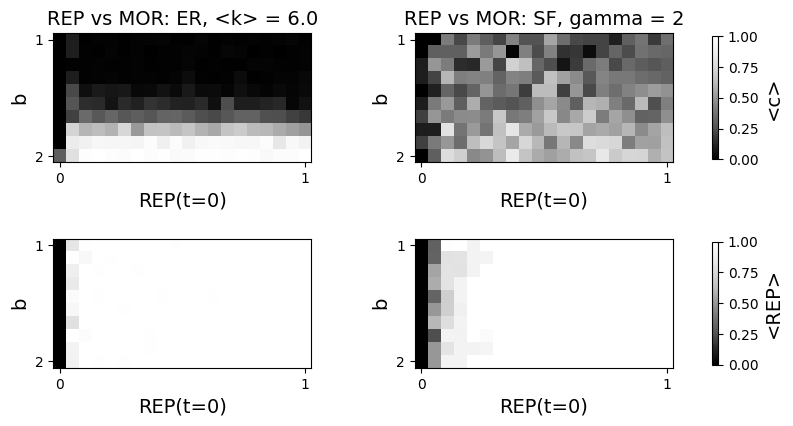
\includegraphics[width=0.8\textwidth]{mat1.png}
	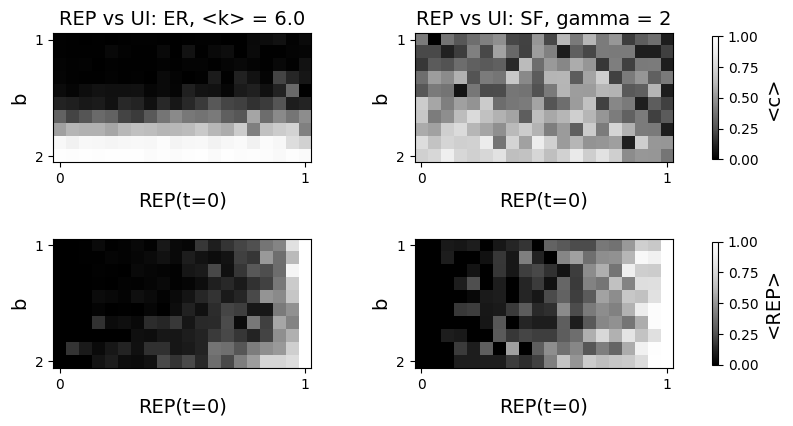
\includegraphics[width=0.8\textwidth]{mat2.png}
	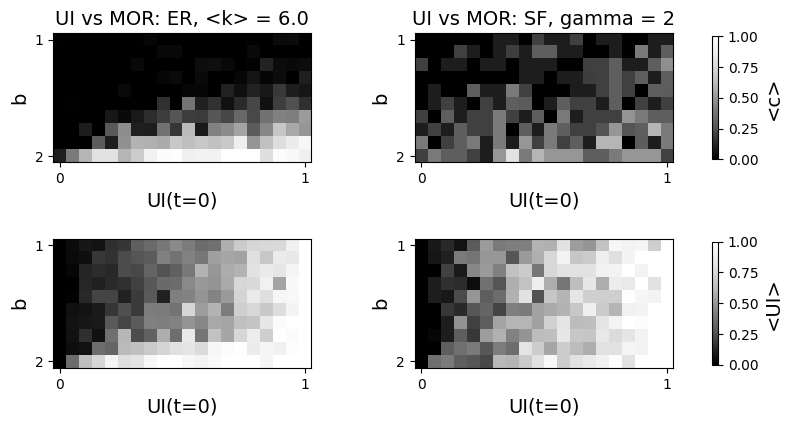
\includegraphics[width=0.8\textwidth]{mat3.png}
 
	\caption{\emph{ Weak prisoners dilema  played by 100 nodes. Played for 1000 iterations or until convergence of UR and STRAT.  Averaged over 10 realizations.}}
	\label{mat}
\end{center}
\end{figure}



\begin{figure}[H]
\begin{center}
	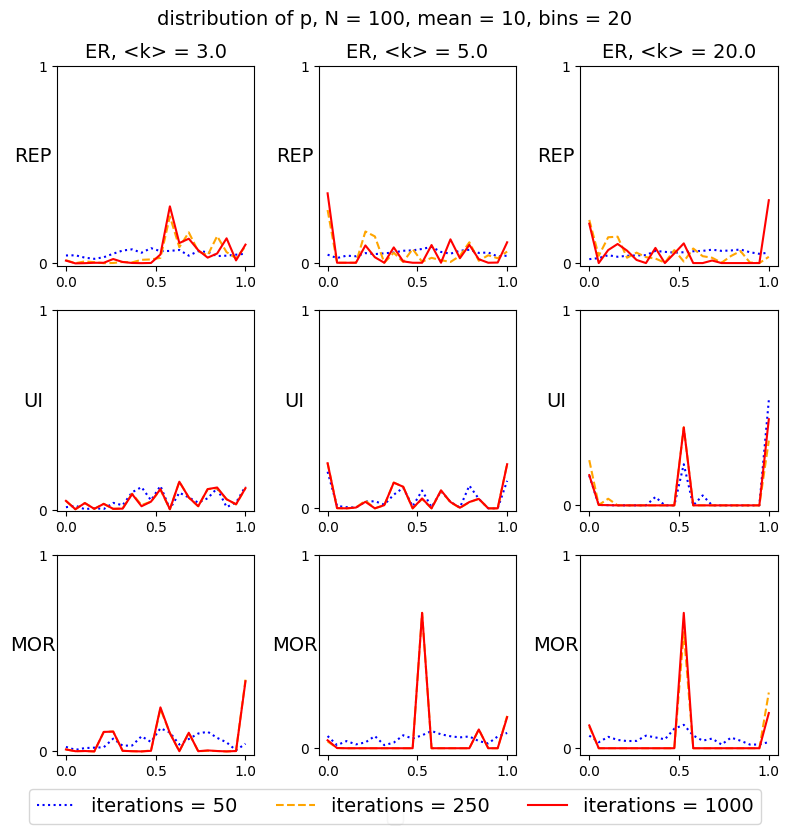
\includegraphics[width=0.7\textwidth]{soc1.png}
	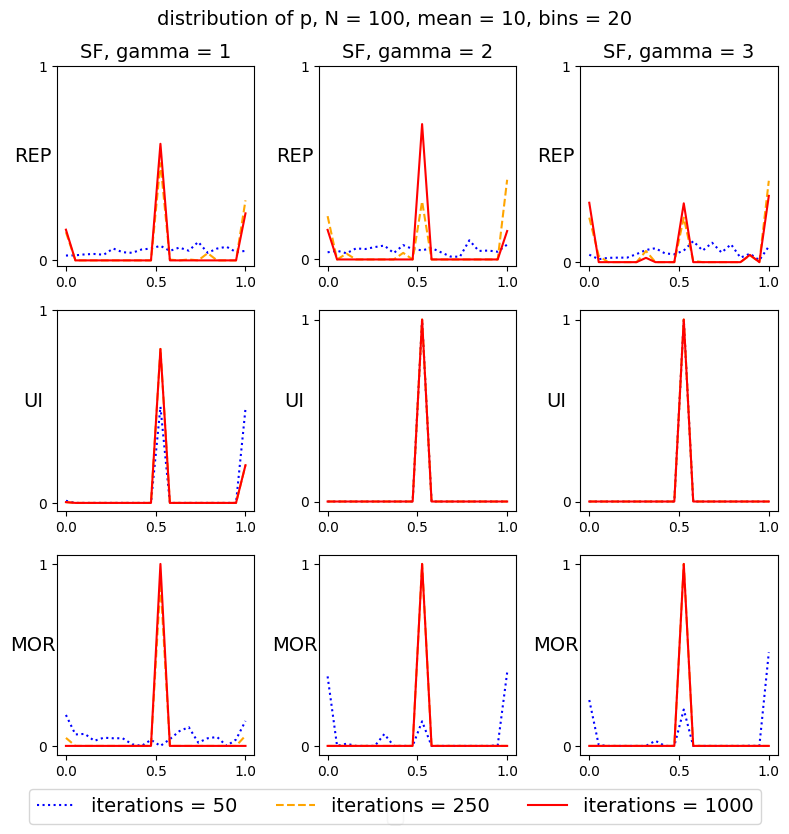
\includegraphics[width=0.7\textwidth]{soc2.png}
 
	\caption{\emph{Ultimatum game without social penalty.  Game played with 100 agents and averaged over 10 realizations. }}
	\label{nosoc1}
\end{center}
\end{figure}
\begin{figure}[H]
\begin{center}
	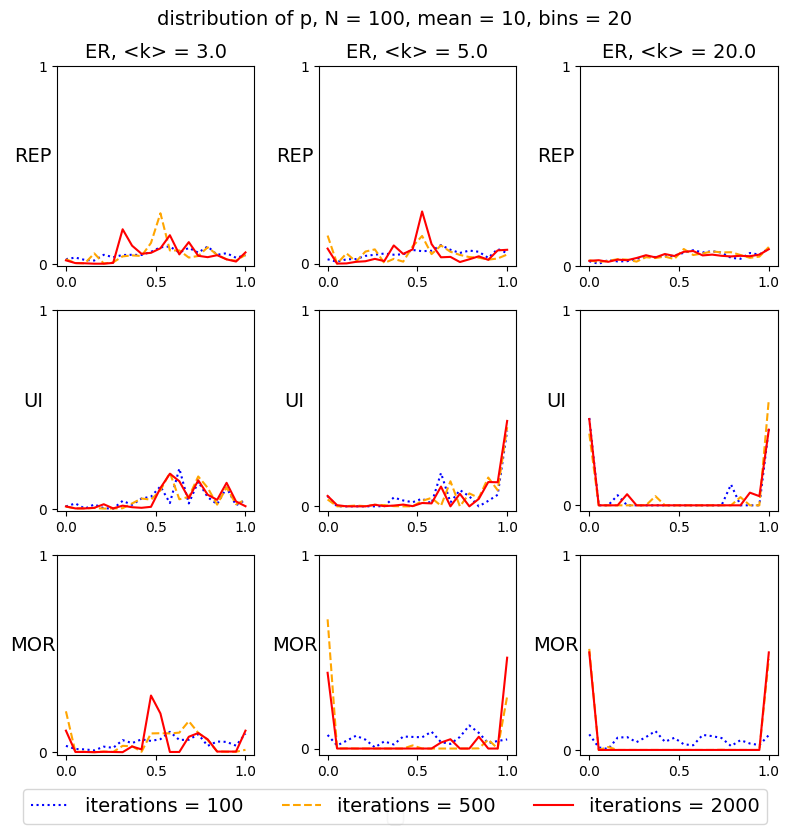
\includegraphics[width=0.7\textwidth]{soc3.png}
	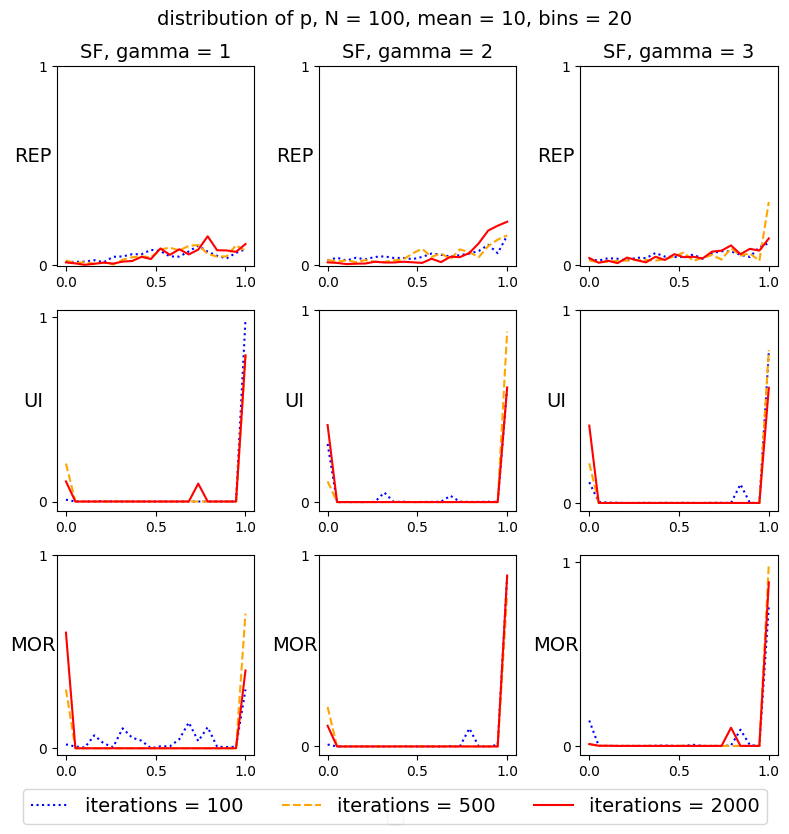
\includegraphics[width=0.7\textwidth]{soc4.png}
 
	\caption{\emph{ Ultimatum game with social penalty.  Game played with 100 agents and averaged over 10 realizations. }}
	\label{nosoc2}
\end{center}
\end{figure}

\newpage